
\setchapterimage[6cm]{cabecera}
\setchapterpreamble[u]{\margintoc}
%%%%%%%%%%%%%%%%%%%%%%%%%%%%%%%%%%%%%%%%%%%%%%%%%%%%%%%%%%%%%

\chapter{Comunicación entre Procesos Remotos }
\label{ch:Comunicación entre Procesos}
\index{comunicación entre procesos}

Este capítulo continua el estudio de los protocolos para la comunicaión entre procesos. Se detallan el Protocolo Soliciud Respuesta, Llamadas a Procedimientos Remotos e Invocación a Métodos Remotos.

\section{Protocolo Solicitud-Respuesta}
\label{sec:sol-resp}
\index{protocolo solicitud respuesta}

El protocolo solicitud-respuesta  está diseñada para apoyar los roles e intercambios de mensajes en interacciones cliente-servidor. El \gls{protocolo solicitud-respuesta} que se describe en la figura \ref{fig:sol-resp}, \cite{Steen2017} \cite{Coulouris2011},  se basa en un trío de primitivas de comunicación: \textit{doOperation},\textit{getRequest} y \textit{sendReply}:

\begin{itemize} 
	\item \textit{doOperation}: los clientes invocan operaciones remotas. Sus argumentos especifican el servidor remoto y la operación a invocar, junto con información adicional (argumentos) requerida por la operación. 
	%%	Su resultado es una matriz de bytes que contiene la respuesta. Se supone que el cliente que llama a \textit{doOperation} dirige los argumentos en una matriz de bytes y desarma los resultados de la matriz de bytes que es regresada.  	Después de enviar el mensaje de solicitud, \textit{doOperation} invoca recibir para obtener un mensaje de respuesta, del cual extrae el resultado y lo devuelve al que llamo. El enlace de \textit{doOperation} se bloquea hasta que el servidor realiza el pedido operación y transmite un mensaje de respuesta al proceso del cliente
	
	\item \textit{getRequest} es utilizado por un proceso de servidor para adquirir solicitudes de servicio.  Envía un mensaje de solicitud al servidor remoto y devuelve la respuesta.   
	
	\item \textit{sendReply} Cuando el servidor ha invocado la operación especificada, usa \textit{sendReply} para enviar el mensaje de respuesta al cliente.
	Cuando el cliente recibe el mensaje de respuesta \textit{doOperation} original se desbloquea y la ejecución del programa cliente continúa.   
\end{itemize}

Ejemplo del protocolo solicitud-respuesta es \textbf{HTTP}  y \textbf{TCP stream} (\cite{Vitillo2021}, \cite{Coulouris2011}).


\begin{figure}%
	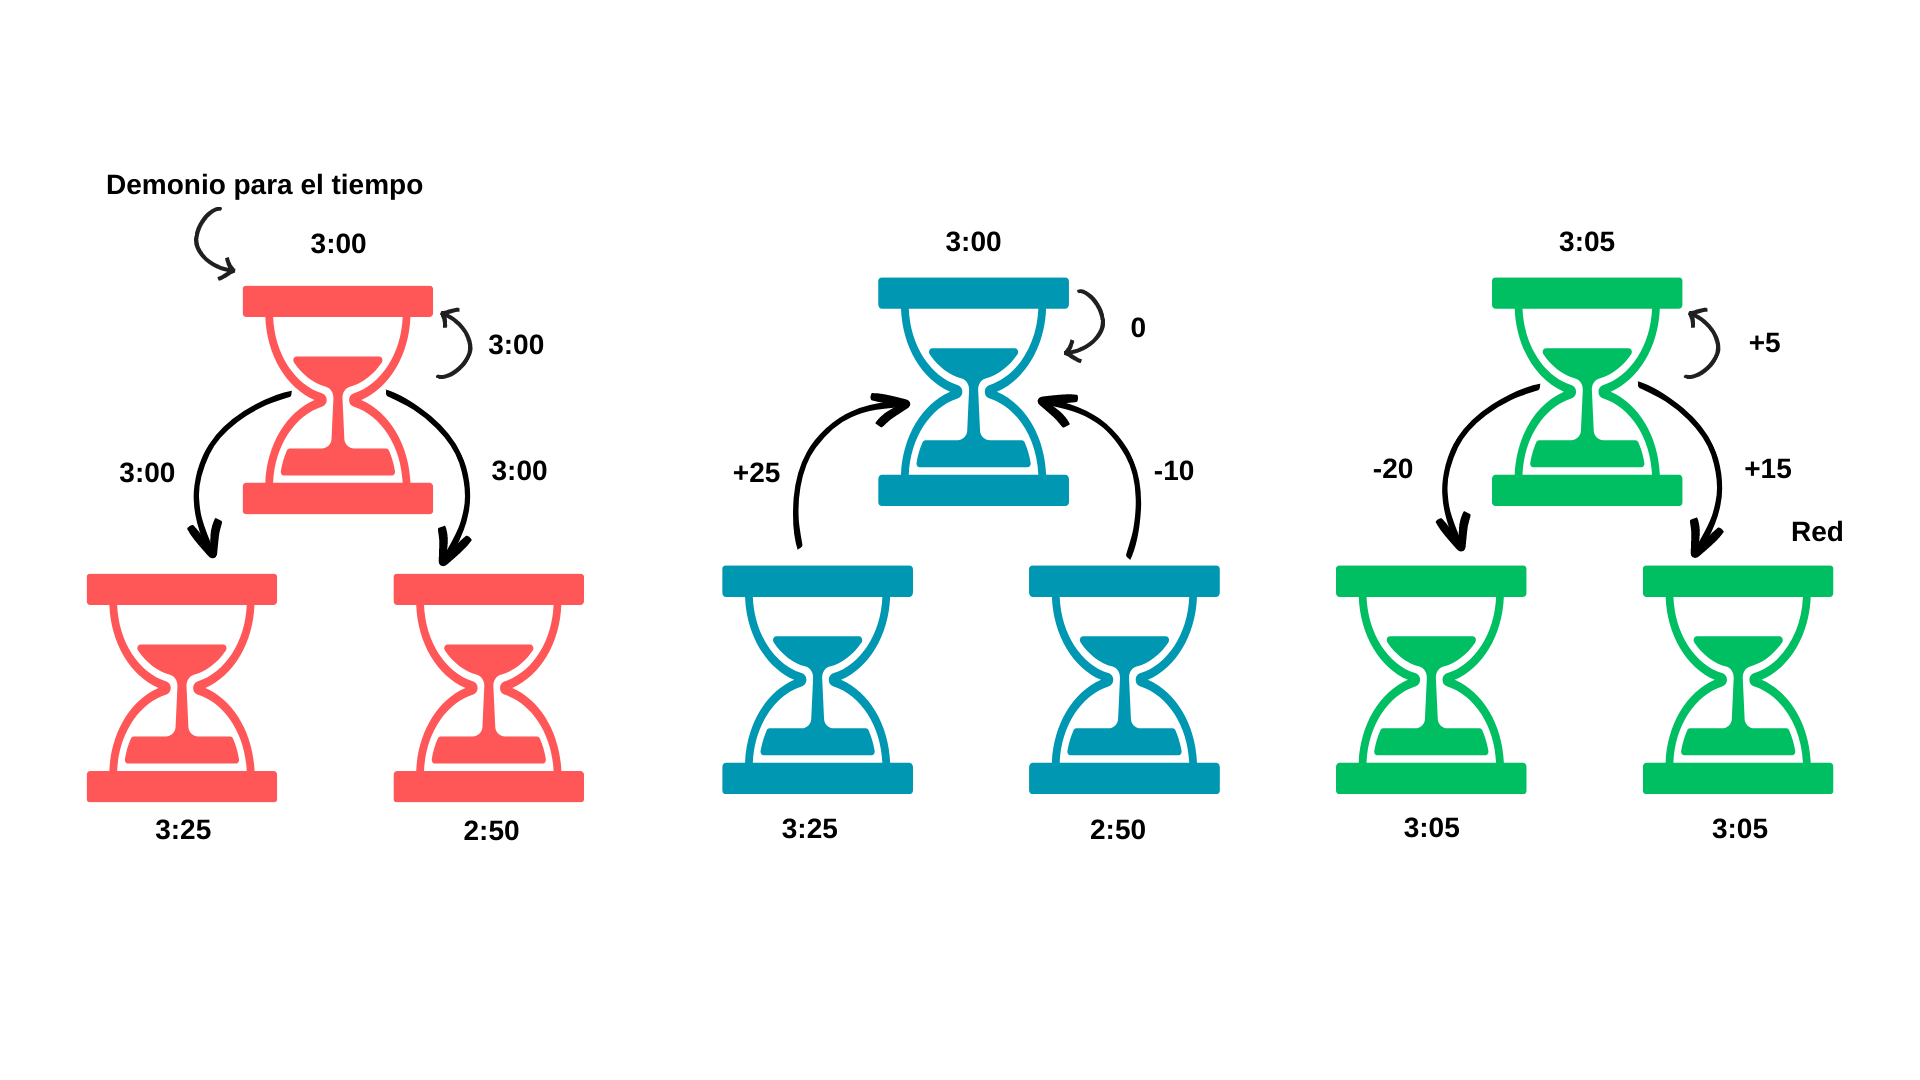
\includegraphics{5/1}   %[width=0.8\textwidth]
	\caption{Protocolo Solicitud Respuesta.}
	\label{fig:sol-resp}
\end{figure}

\subsection{Estructura del Mensaje}  \index{estructura del mensaje}

La información a transmitir en un mensaje del protocolo solicitud-respuesta,  se muestra en la figura \ref{fig:est-men}


\begin{figure}%
	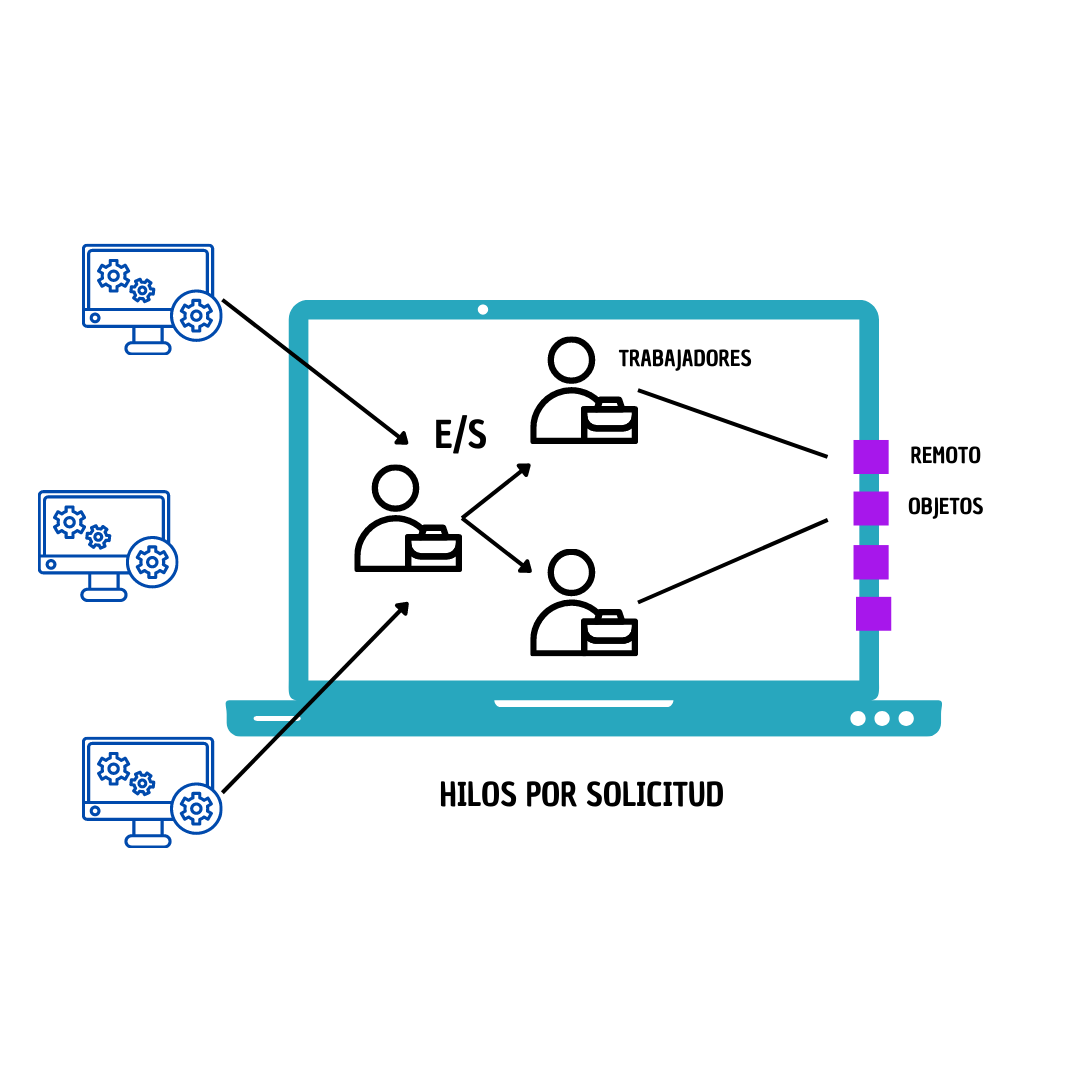
\includegraphics{5/2}     % [width=0.8\textwidth]
	\caption{Estructura del mensaje.}
	\label{fig:est-men}
\end{figure}

\begin{itemize}
	\item El primer campo indica si el mensaje es una Solicitud o un mensaje de Respuesta
	\item El campo\textit{requestId}, contiene un identificador de mensaje generado por una  operación en el cliente por cada mensaje de solicitud;  el servidor copia estos \textit{ID} en los mensajes de respuesta correspondientes. Esto permite que \textit{doOperation} verifique que la respuesta es el resultado de la solicitud actual. 
	\item El tercer campo es una referencia remota, es el identificador del objeto remoto.
	\item El cuarto campo es el conjunto de argumentos que definen las operaciones que se van  a invocar.
\end{itemize}


\subsection{Fallas}  \index{modelo fallas}

Si el protocolo solicitud-respuesta se implementan sobre datagramas\textit{UDP},  entonces sufren de los mismos fallos de comunicación que \textit{UDP}. Es decir:
\begin{itemize}
	\item Fallas por omisión del mensaje. 
	\item No se garantiza que los mensajes se entreguen en el orden del remitente.
\end{itemize}

  
\subsection{Características del Protocolo solicitud-respuesta}
 
 \index{caracter\'isticas del protocolo solicitud-respuesta}
 
\begin{itemize}
	\item \textbf{Tiempos de Espera.} Para las  ocasiones en  que un servidor  falla o que  se descarta una solicitud o un mensaje de respuesta,  la \textit{doOperation} usa un \textit{timeout} mientras está esperando obtener  mensaje de respuesta del servidor. Para compensar la posibilidad de pérdida de mensajes,  \textit{doOperation} puede reenvíar el mensaje de solicitud repetidamente hasta que recibe una respuesta.
	
	\item \textbf{Mensajes Duplicados.} En los casos en que el mensaje de solicitud sea  retransmitido, el servidor puede recibirlo más de una vez. %%Por ejemplo, el servidor puede  recibir el primer mensaje de solicitud, pero tomar más tiempo que el tiempo de espera del cliente para ejecutar el 	comando y devolver la respuesta. 
	Esto puede llevar a que el servidor ejecute una operación más  de una vez para la misma solicitud. Para evitar esto, el protocolo está diseñado para reconocer  mensajes sucesivos (del mismo cliente) con el mismo identificador de solicitud, para filtrar los duplicados. 
	
	\item \textbf{Mensajes Perdidos.} Si el servidor ya ha enviado la respuesta cuando recibe una solicitud duplicada, deberá ejecutar la operación nuevamente para obtener el resultado , a menos que haya almacenado el resultado de la ejecución original.  %(\gls(idempotente))
	
	\item \textbf{Historial.}
	Para los servidores que requieren una retransmisión de respuestas sin repetir la  ejecución de las operaciones, se puede usar  un \texttt{historial} de los mensajes transmitidos.
	Una entrada en un \texttt{historial} contiene un identificador de solicitud, un mensaje y un identificador del cliente al que se envió la respuesta. Su propósito es permitir que el servidor retransmita los mensajes de respuesta cuando los procesos del cliente los soliciten. 
\end{itemize}
 

\subsection{Estilos del protocolo}   \index{estilos de protocolos}

Se pueden describir tres estilos de protocolos relacionados al protocolo Solicitud-Respuesta, que producen diferentes comportamientos:
\begin{itemize}
\item El protocolo Solicitud (R). El cliente envía un mensaje de solicitud único al servidor.  El cliente puede procesar inmediato después de que se envíe el mensaje de solicitud, ya que no es necesario esperar un mensaje de respuesta. Este protocolo se implementa a través de los datagramas de UDP y, además, sufre de las mismas falles de comunicación.



\item  El protocolo de solicitud-respuesta (RR). El protocolo RR es útil para la mayoría de los intercambios de clientes-servidores. No se requieren mensajes de acuse de recibo especial, ya que el mensaje de respuesta de un servidor se considera un acuse de recibo del mensaje de solicitud del cliente. 


\item   El protocolo  Solicitud-Respuesta (RRA).  El protocolo RRA se basa en el intercambio de tres mensajes: Solicitud, respuesta y reconocimiento. El mensaje de reconocimiento    contiene el \textit{requestId} del mensaje de  respuesta. Esto permitirá al servidor descartar las entradas de su historial. 
\end{itemize}


%%%%%%%%%%%%%%%%%%%%%%%%%%%%%%%%%%%%%%%%%%%%%%%%%%%%%%%%%%%%%%%%%%%%%%%%%%%%%%%%%%%%%%%%%%%%%%%%%%%%%%%%%%%%%%%%%%%%%%%%%%%%%%%%%%%%%%%%%%%%%%%%%%%%%%%%%%%%%%%5
 

\section{Llamados a Procedimientos Remotos (RPC)}
\label{sec:RPC}
\index{RPC}

Se analizan tres aspectos que son importante para comprender este concepto:
\begin{itemize}
	\item el estilo de programación promovido por RPC - programación con interfaces;
	\item la semántica de llamadas asociada con RPC;
	\item  la transparencia y su relación con las llamadas a procedimientos remotos.
\end{itemize}

\subsection{Programaci\'on con Interfases}
\index{programaci\'on con interfases}

La interfaz de un módulo especifica los procedimientos y las variables a las que se pueden acceder a trav\'es de  otros módulos. 
En sistemas distribuidos las interfaces son  programas distribuidos donde los módulos se ejecutan en procesos separados.
En el modelo cliente-servidor, en particular, cada servidor proporciona un conjunto de procedimientos que están disponibles para uso de los clientes, \sidecite{Vitillo2021} \sidecite{Coulouris2011}.
\begin{itemize}
	\item No hay detalle de implementación lenguaje de programación. Hay una evolución del software
	\item No hay acceso a variables mediante ejecución de procesos remotos ni mecanismos pase de parámetros (llamada por valor o referencia)
	\item  Direcciones en procesos locales no son válidas en los procesos remotos
	
	\item  Mecanismo RPC se integra con el lenguaje de programación e incluye la notación  para la definición de interfaces con mensajes input/output
	\item Escrita en variedades de lenguajes, C++, Java, Python
	\item Lenguajes de definición de interfaces (IDL) están diseñados para permitir que los procedimientos implementados en distintos lenguajes puedan ser invocados por otros
	
\end{itemize}

\subsection{Semántica de llamadas de RPC}
\index{sem\'antica de llamadas RPC}

La operaci\'on \textit{doOperation} se puede implementar de diferentes maneras para proporcionar diferentes garantías de entrega en el mensaje (figura \ref{tab:RPC-Semant}). Las principales opciones son:
\begin{itemize}
	\item Reintentar mensaje de solicitud: controlar si se retransmite el mensaje de solicitud hasta se recibe una respuesta o supone que el servidor ha fallado. 
	\item Filtrado duplicado: controlar cuándo se usan las retransmisiones y si se debe filtrar solicitudes duplicadas en el servidor. 
	\item Retransmisión de resultados: controlar si se debe mantener un historial de mensajes de resultados para permitir que los resultados perdidos se retransmitan sin volver a ejecutar las operaciones en el servidor.
\end{itemize}

 
%%%%%%%%%%%%%%%%%%%%%%%%%%%%%%%%%%%%%%%%%%%
 
\definecolor{LightCyan}{rgb}{0.88,1,1}

\begin{table}[h] 
%	\footnotesize%
	\begin{center}
		\footnotesize
	%	\scriptsize
		\begin{tabular}{p{0.25\linewidth}p{0.2\linewidth}p{0.2\linewidth}p{0.2\linewidth}}			
			\toprule
			\rowcolor{LightCyan} 
		\multicolumn{3}{c}{Medidas de Tolerancia de Fallas}	 & Sem\'antica de Llamadas  \\
			\midrule 
			\quad \cellcolor{LightCyan} Retransmisi\'on mensaje  & \cellcolor{LightCyan} Filtrado de duplicados & \cellcolor{LightCyan} Re-ejecuci\'on o retransmisi\'on de mensajes & \\ 
			\hline
			\\
			\quad No  & No aplica &  No aplica & Puede ser \\  \\
			\quad Si  & No  & Re-ejecuci\'on & Al-menos-una-vez \\  \\
			\quad Si  & Si  &  Retransmisi\'on de la respuesta & como-máximo-una-vez \\	
			\addlinespace 
			\bottomrule		
		\end{tabular}
	\end{center}
	\caption{Sem\'antica de Llamadas RPC.  Adaptado de \CO }
	\label{tab:RPC-Semant}
\end{table}

%%%%%%%%%%%%%%%%%%%%%%%%%%%%%%%%%%%%%%%%

Por ejemplo, con una semántica \textbf{Puede-ser}, el invocador de la llamada recibe un resultado, en cuyo caso el invocador de la llamada  sabe que el procedimiento se ejecutó al menos una vez, o una excepción que le informa que no se recibió ningún resultado. 
La semántica \textbf{Al-menos-una-vez}, puede ser lograda mediante la retransmisión de mensajes de solicitud, que enmascara las fallas de omisión del mensaje de solicitud o resultado. 
La semántica puede sufrir lo siguiente tipos de falla:
\begin{itemize}
	\item fallas de bloqueo cuando falla el servidor que contiene el procedimiento remoto;
	\item fallas arbitrarias: en los casos en que el mensaje de solicitud se retransmite,  el servidor puede recibirlo y ejecutar el procedimiento más de una vez, posiblemente causando valores incorrectos para ser almacenados o devueltos.
\end{itemize}

Con una semántica \textbf{como-máximo-una-vez}, la persona que llama recibe un resultado, en cuyo caso la persona que llama sabe que el procedimiento se ejecutó exactamente una vez, o una excepción que le informa que no se recibió ningún resultado, entonces el procedimiento ha sido ejecutados ya sea una vez o no lo ha sido.


\subsection{Transparencia}
\index{transparencia en RPC}
La elección de si el RPC debe ser transparente también está disponible para los diseñadores de IDL. Por ejemplo, en algunos IDL, una invocación remota puede generar una excepción cuando el cliente no puede comunicarse con un procedimiento remoto. Esto requiere que el programa cliente maneje tales excepciones, permitiéndole lidiar con tales fallas. Un IDL también puede proporcionar una facilidad para especificar la semántica de llamada de un procedimiento. Esto puede ayudar al diseñador del servicio; por ejemplo, si se elige la semántica de llamada al menos una vez para evitar los gastos generales de una vez como máximo, las operaciones deben diseñarse para que sean idempotentes.

%\begin{figure}% %%	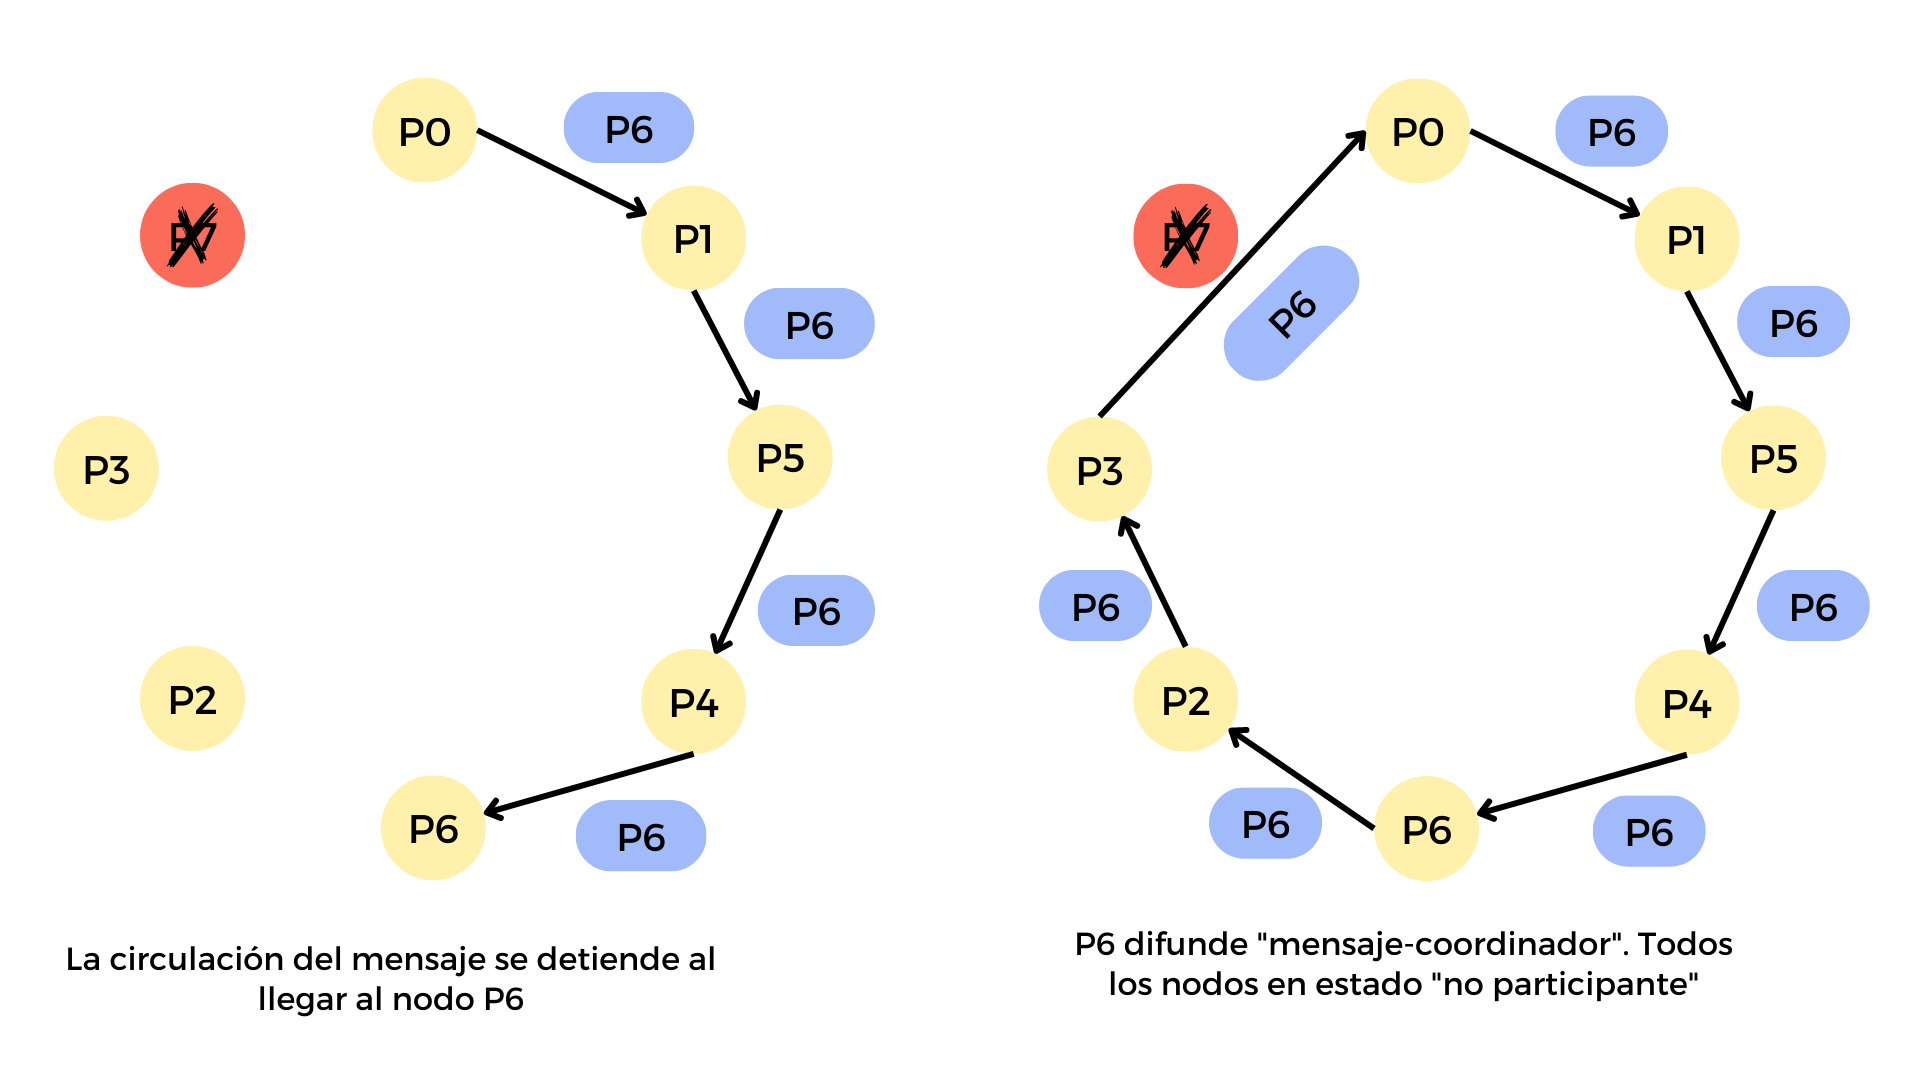
\includegraphics {5/4} 	\caption{.} 	\label{fig:RPC-2} \end{figure}

\subsection{Implementaci\'on de RPC}
\index{implementaci\'on de RPC}
La llamada a procedimiento remoto (RPC) es una técnica orientada a la construcc\'on  de aplicaciones distribuidas basadas en cliente-servidor. Se basa en la extensión de la llamada de procedimiento local  de manera que el procedimiento llamado no necesita existir en el mismo espacio de direcciones que el procedimiento de llamada. Los dos procesos pueden estar en el mismo sistema, o pueden estar en diferentes sistemas con una red que los conecta.


\begin{figure}%
	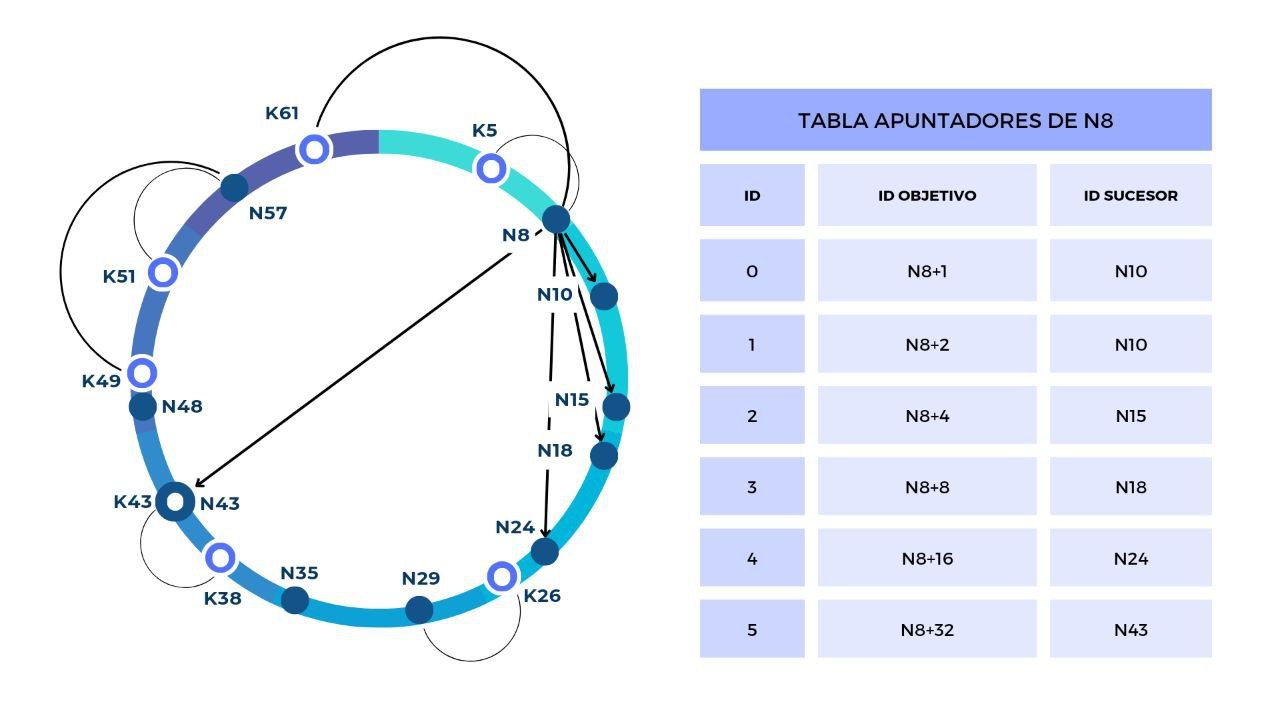
\includegraphics {5/3}
	\caption{Llamada a Procedimiento Remoto.}
	\label{fig:RPC-1}
\end{figure}

En la figura \ref{fig:RPC-1} se muestra lo que ocurre cuando se hace una llamada a un proceso remoto:
\begin{enumerate}
	\item El entorno de llamada se suspende, los parámetros del procedimiento se transfieren a través de la red al entorno donde se ejecutará el procedimiento.
	\item Cuando finaliza el procedimiento y produce sus resultados, estos se transfieren de vuelta al entorno de llamada, donde se reanuda la ejecución como si regresara de una llamada de procedimiento regular.
	
\end{enumerate}

El la figura \ref{fig:rpc} se muestra un esquema de los componentes de la arquitectura de RPC.

El cliente que accede a un servicio incluye un procedimiento \textit{stub} para cada procedimiento definido en la interfaz de servicio. El procedimiento \textit{stub} se comporta como un procedimiento local para el cliente, pero en lugar de ejecutar la llamada, ordena (empaqueta) el identificador del procedimiento y los argumentos en un mensaje de solicitud, que envía a través de su módulo de comunicación al servidor. 

Cuando llega el mensaje de respuesta, el  módulo de comunicación  desarma (desempaqueta) los resultados. El proceso del servidor contiene un despachador junto con un procedimiento de código auxiliar del servidor y un procedimiento de servicio para cada procedimiento en la interfaz de servicio. El despachador selecciona uno de los procedimientos \textit{stub}  del servidor, según el identificador de procedimiento en el mensaje de solicitud. 

El procedimiento de \textit{stub} del servidor luego  desarma (desempaqueta)  los argumentos en el mensaje de solicitud, llama al procedimiento del servicio correspondiente  y calcula los valores de retorno para el mensaje de respuesta. 

Los procedimientos de servicio implementan los procedimientos en la interfaz de servicio. Los procedimientos de \textit{stub} de cliente y servidor y el despachador puede ser generado automáticamente por un compilador de interfaz a partir de la definición de interfaz del servicio.

 RPC puede implementarse para tener una de las opciones de semántica de invocación o llamadas, generalmente se elige al menos una vez o como máximo una vez. Para lograr esto, el módulo de comunicación implementará las opciones de diseño deseadas en términos de retransmisión de solicitudes, tratamiento de duplicados y retransmisión de resultados.


\begin{figure}%
	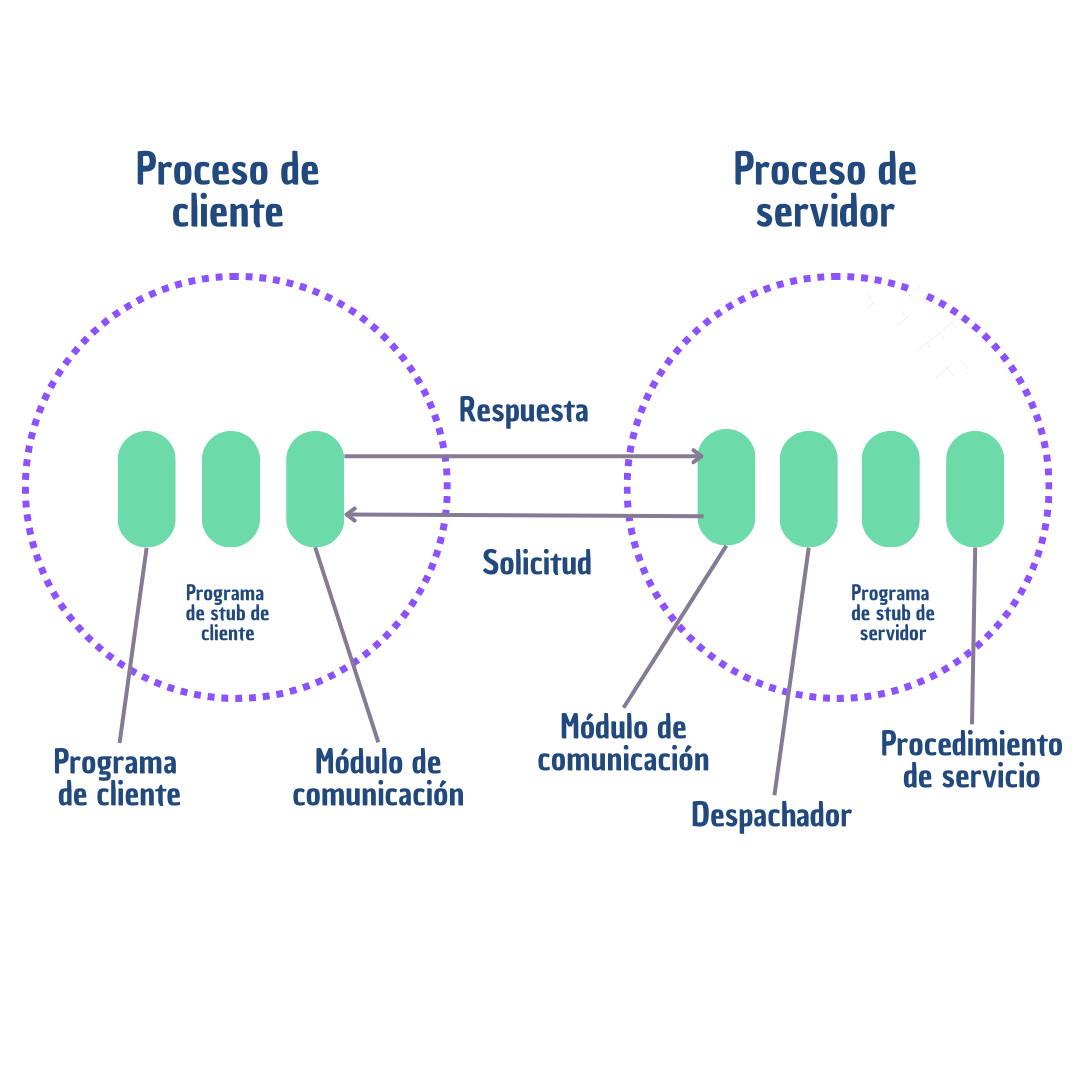
\includegraphics {5/5}
	\caption{Arquitectura de RPC}
	\label{fig:rpc}
\end{figure}
%%%%%%%%%%%%%%%%%%%%%%%%%%%%%%%%%%%%%%%%%%%%%%%%%%%%%%%%%%%%%%%%%%%%%%%%%%%%%%


\section{Invocaci\'on a M\'etodos Remotos (RMI)}
\index{RMI}

Los puntos en común entre RMI y RPC son los siguientes:
\begin{itemize}
	\item Ambos admiten programación con interfaces.
	\item  Están construidos sobre protocolos de solicitud-respuesta y pueden ofrecer un rango de semántica de llamadas como al menos una vez y como máximo una vez.
	\item Ambos ofrecen un nivel similar de transparencia, es decir, las llamadas locales y remotas emplean la misma sintaxis, pero las interfaces remotas suelen exponer la distribución de la llamada subyacente, por ejemplo, admitiendo excepciones remotas.
	
\end{itemize}

Las siguientes diferencias conducen a una mayor expresividad cuando se trata de programación de aplicaciones y servicios distribuidos complejos:

\begin{itemize}
	
	\item El programador puede utilizar todo el poder expresivo de la programación orientada a objetos para  el desarrollo de software de sistemas distribuidos.
	
	\item  Todos los objetos en un sistema basado en RMI tienen referencias de objeto únicas (ya sean locales o remoto), tales referencias de objeto también se pueden pasar como parámetros, ofreciendo así semántica de paso de parámetros significativamente más rica que en RPC.
\end{itemize}



Los siguientes  conceptos  están presentes en el modelo de objeto distribuido: 
\begin{itemize}
	\item Referencias a objetos remotos: otros objetos pueden invocar los métodos de un objeto remoto si tienen acceso a su referencia de objeto remoto. \index{referencia a objetos remotos}
	\item  Interfaces remotas: cada objeto remoto tiene una interfaz remota que especifica qué de sus métodos se pueden invocar de forma remota.  \index{interfases remotas}
\end{itemize}


\subsection{Arquitectura RMI}
\index{arquitectura de RMI}

La arquitectura se muestra en la figura \ref{fig:rmi} (\sidecite{Vitillo2021},   \sidecite{Verissimo2012}, \sidecite{Coulouris2011}):

\begin{description}
	 
	\item[Módulo de Comunicación] Proporcionan semántica de invocación, como ejemplo, al-menos-uno
	Transmite mensaje de solicitud/respuesta entre cliente y servidor
	Solicitud es (tipo de mensaje, IdSolicitud, ref objeto remoto, IdOperacion, Argumentos)
	En el servidor selecciona el despachador para la clase de objeto que se invoca. 
	El despachador ubica la referencia local del objeto en el Módulo de Referencia Remota
	
	
	\begin{figure}%
		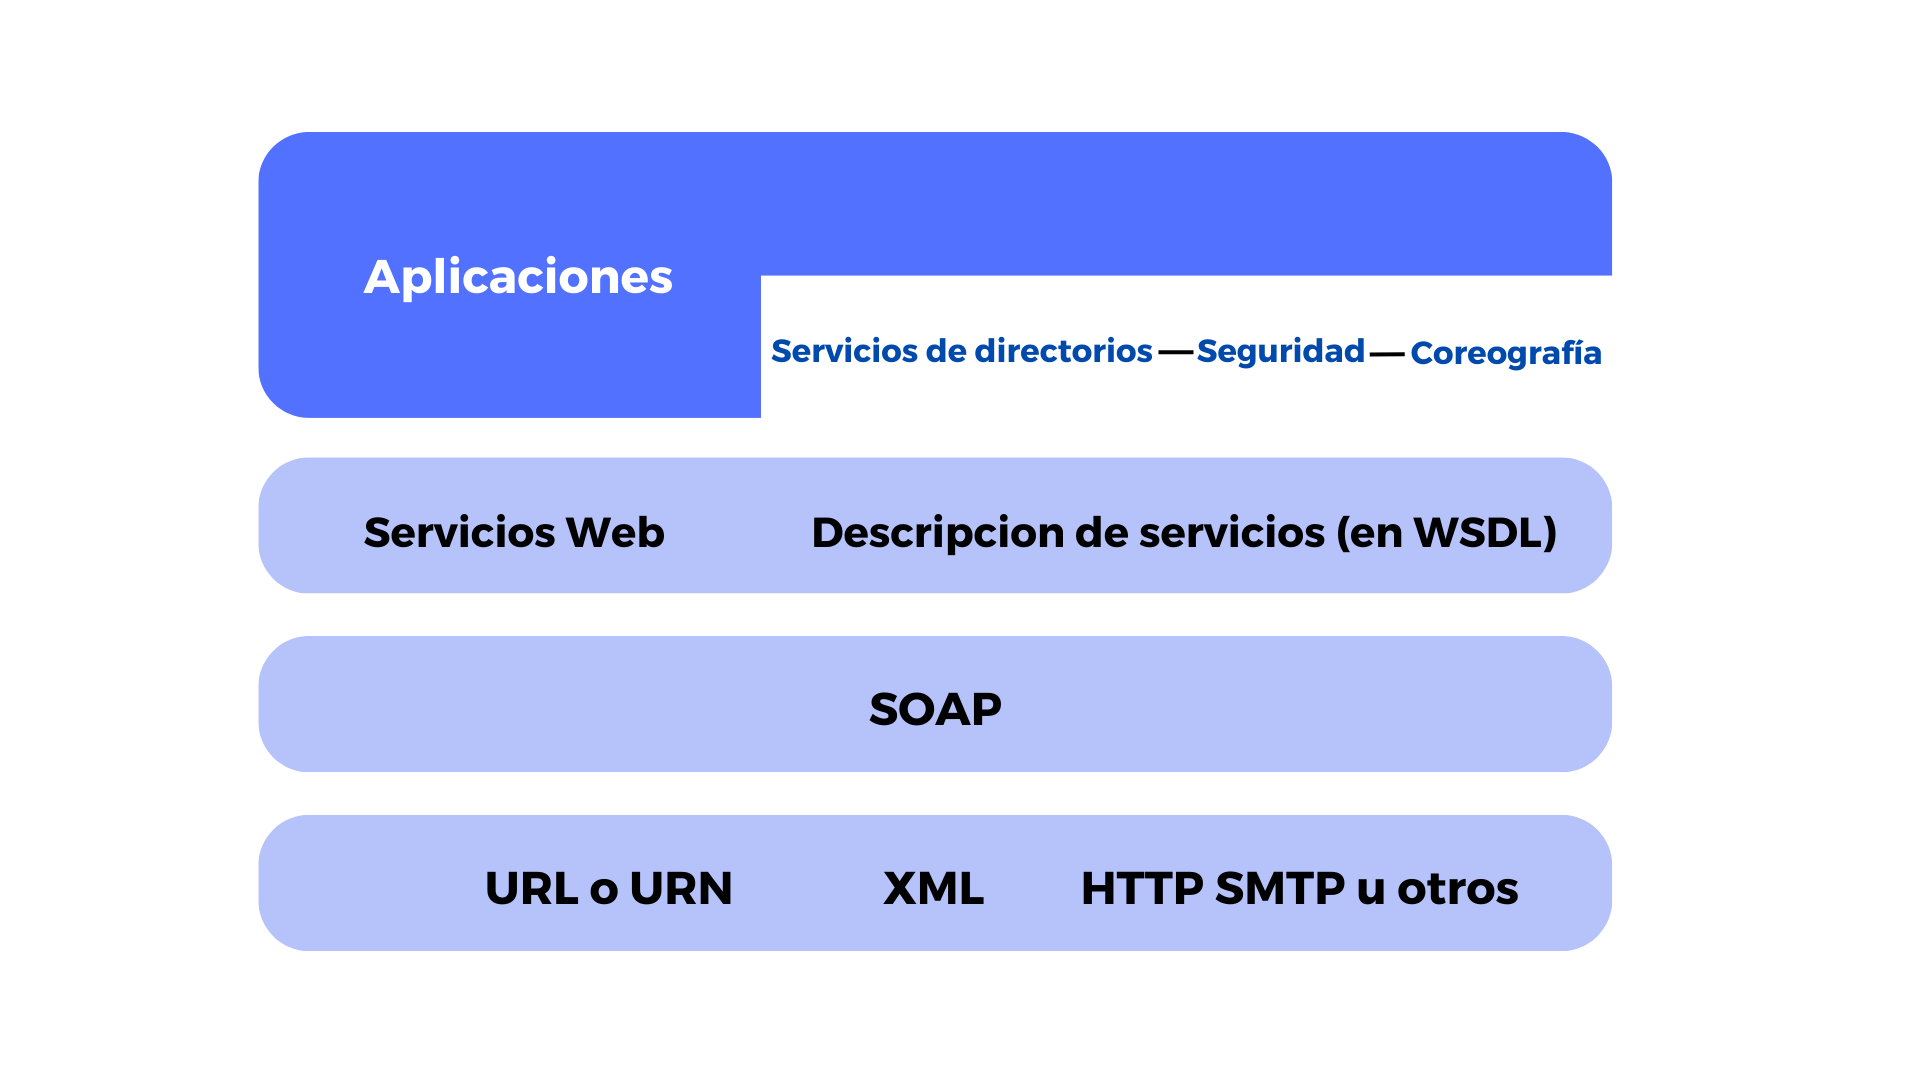
\includegraphics {5/6}
		\caption{Arquitectura RMI.}
		\label{fig:rmi}
	\end{figure}
	
	\item[Módulo de Referencia Remota] Responsable de trasladar referencias de objetos locales a remotas y creación de referencias remotas
	Contiene una  tabla de objetos remotos y una tabla para cada proxy local
	Actúa de la manera siguiente:
	\begin{itemize}
		\item 1era vez cuando se pasa un objeto remoto, el módulo de referencia remota crea una referencia al objeto remoto y se añade a la tabla de objetos remotos
		\item Cuando llega referencia a un objeto remoto, el módulo de referencia obtiene referencia al objeto local, la cual es un proxy o un objeto remoto. Si el objeto remoto no está en la tabla se crea el proxy y se añade el módulo de referencia remota
	\end{itemize}
	
	\item[Criado (servant)] Instancia de una clase que proporciona el cuerpo de un objeto remoto. 
	Maneja el requerimiento remoto pasado por el esqueleto              correspondiente. Se crea cuando se instancia el objeto remoto. 
	
	\item[Proxy]
	Proporciona que los métodos de invocación remota sean                 transparente al usuario comportandose como un objeto local.
	Esconde los detalles del empaquetamientos- desempaquetamiento de las referencias a objetos remotos.
	
	\item[Despachador] 
	Un servidor tiene un despachador y un esqueleto.
	Recibe la petición desde el  módulo de comunicación.
	Usa el IdOperacion para seleccionar el método adecuado en el esqueleto
	
	\item[Esqueleto] 
	Implementa el método  en la interface remota. 
	Desempaqueta los argumentos e invoca el método      				correspondiente en el criado.
	Espera que la invocación se complete y empaqueta los resultados
\end{description}


\subsection{Colector de Basura Distribuida} 
\index{colector de basura distribuida}
Es un algoritmo distribuido cuya funci\'on es  recolectar la basura distribuida. Establece una cooperación entre el colector local y un módulo añadido que colecciona la basura distribuida

Colector de basura distribuida:
\begin{enumerate}
	\item  Cada proceso servidor mantiene un conjunto de nombres de los procesos que proporcionan referencias a objetos remotos por cada uno de sus objetos remotos. Este conjunto se puede almacenan en una columna adicional de la tabla de objetos remotos.
	\item Cuando un cliente C recibe una referencia remota a un objeto remoto en particular, B,  hace una invocación AddRef (B) al servidor de ese objeto remoto y luego crea un proxy; el servidor agrega un apuntador C a B.
	\item  Cuando  recolector de basura de un cliente C nota que un proxy de un objeto remoto B no está accesible, hace una invocación removeRef (B) al servidor correspondiente y luego borra el proxy; el servidor elimina apuntador C de B.
	\item Cuando apuntador B está vacío, el recolector de basura local del servidor recuperará el espacio ocupado por B a menos que existan apuntadores locales.
\end{enumerate}

\section{Caso de Estudio: API}
\index{caso de estudio!API}

Las tecnologías de comunicación entre procesos más utilizadas para las interacciones de solicitud y respuesta son \textbf{RPC}, \textbf{REST} y \textbf{GraphQL}. Por lo general, las API internas que se usan para las comunicaciones de servicio a servicio dentro de una organización se implementan con un marco RPC de alto rendimiento como gRPC.

\marginnote[-4.2cm]{
	\begin{kaobox}[frametitle=gRPC]
		gRPC, Google Remote Procedure Call,  es un sistema de llamada a procedimiento remoto de código abierto desarrollado inicialmente en Google. 	
	\end{kaobox}   }

Por el contrario, las API externas disponibles para el público tienden a basarse en \textbf{REST}  o \textbf{GraphQl}. En lo que queda, presentaremos estas tecnolog\'ias.

\subsection{ ?`Que es un API?}
 
Un desarrollador usa una \gls{API} cuando escribe software que interactuará con un sistema de software externo cerrado. El sistema de software externo proporciona una API como un conjunto estándar de herramientas que todos los desarrolladores pueden usar. Ejemplos  son las APIs de  Google,  YouTube, Twitter, entre otras. 

\subsection{ ?`Que es REST?}
\index{Rest}
\index{RestFul}

\textbf{REST} (REST, Representational State Transfer) es un estilo de arquitectura de software propuesto por \sidecite{Fielding2000}. 
\textbf{REST} es una arquitectura orientada a los recursos en la que los usuarios gestionarían los recursos web realizando operaciones HTTP como GET, PUT, POST y DELETE. La red de recursos se puede considerar como una máquina de estado virtual y las acciones (GET, PUT, POST, DELETE) son cambios de estado dentro de la máquina. 
Esto significa  que cuando se usa el paradigma \textbf{REST} para construir un \textbf{API REST}, se tiene un medio uniforme para crear, leer y actualizar datos usando \textbf{URL HTTP} simples con un conjunto estándar de verbos \textbf{HTTP} \sidecite{Satheesh2015}, \sidecite{Erl2013}.

Mientras \textbf{REST} esta relacionado con una serie de restricciones, el t\'ermino \textit{\textbf{RESTful}} hace referencia a un API que se adhiere a los siguientes criterios:

\begin{itemize}
	\item Arquitectura cliente-servidor compuesta de clientes, servidores y recursos, con la gestión de solicitudes a través de HTTP.
	\item Comunicación entre el cliente y el servidor \gls{sin estado} (\textit{stateless}).
	\item Uso del \textbf{caché} para almacenar datos  y optimizar las interacciones entre el cliente y el servidor.
	\item Una interfaz uniforme entre los elementos, para que la información se transfiera de forma estandarizada: recursos identificables de manera que el cliente pueda manipularlos.
	\item Un sistema en capas que organiza en jerarquías  cada uno de los servidores (los encargados de la seguridad, del equilibrio de carga, etc.) y que participan en la recuperación de la información solicitada.
	\item\gls{Codigo por demanda}, es decir, a solicitud del cliente. 
\end{itemize}

 
Cuando el cliente envía una solicitud a través de una API de RESTful, esta transfiere una representación del estado del recurso requerido a quien lo haya solicitado o al extremo. La información se entrega por medio de HTTP en uno de estos formatos: JSON (JavaScript Object Notation), HTML, XLT, Python, PHP o texto sin formato. JSON es el lenguaje de programación más popular, ya que tanto las máquinas como las personas lo pueden comprender y no depende de ningún lenguaje, a pesar de que su nombre indique lo contrario. 


%%\subsubsection*{Hola Mundo con API XMLREST }

\subsection{GraphQl}

\textbf{GraphQL} es un lenguaje de consultas para las API, desde la perspectiva del consumidor  de esas API de datos. La palabra \textit{graph} en \textbf{GraphQL} proviene del hecho de que la mejor manera de representar datos en el mundo real es con una estructura de datos similar a un grafo, \sidecite{Buna2021},  \sidecite{Banks2018}.


Como alternativa a \textbf{REST}, \textbf{GraphQL} permite que los desarrolladores creen consultas para extraer datos de varias fuentes en una sola llamada a la API. \textbf{GraphQL} proporciona un enfoque de API web en el que los clientes definen la estructura de los datos que devolverá el servidor. Esto puede impedir el almacenamiento en caché  de los resultados de la consulta.

\marginnote{
	\begin{kaobox}[frametitle= Problema de API REST]
	Una API REST es una colección de  puntos finales donde cada punto final representa un recurso. Cuando un cliente necesita datos sobre múltiples recursos, tiene que realizar múltiples solicitudes a esa API REST y luego reunir los datos combinando las múltiples respuestas que recibe.	
\end{kaobox}   }
